 % Преамбула
\documentclass[12pt, oneside, dvipsnames]{extarticle}


%вставка изображений и картинок всяких

\usepackage{graphicx}
\newcommand{\incfig}[1]{%
    \def\svgscale{1.5}
    \import{./figures/}{#1.pdf_tex}
}
\graphicspath{{pictures/}}
\DeclareGraphicsExtensions{.pdf,.png,.jpg, .jpeg, .tex}

\usepackage{booktabs} % для таблиц
\usepackage{enumitem} % для списков


% Шрифты

\usepackage[english,russian]{babel}
\usepackage[T1]{fontenc}
\usepackage{libertine}


\usepackage{titling} % для \maketitle
\usepackage{textcomp}% специальные символы в тексте

\usepackage{mathtext}
\usepackage{amsmath,amsfonts,amssymb,amsthm,mathtools} % математика
\usepackage{icomma} % умная запятая
\usepackage{import} %  импортирование


\usepackage{pdfpages} % мультри-пдф страницы
\usepackage{transparent} % что-то про цвета


\usepackage{caption} % комментарии к figure
\usepackage{epigraph} % эпиграфы

\usepackage{comment} % удобные комментарии
\usepackage{xfrac} % дроби
\usepackage{moresize} % все размеры шрифтов
\usepackage{dsfont} % mathbb для всего


% Окружения для математики:

\newtheorem{statement}{Предложение}
\newtheorem{corollary}{Следствие}
\newtheorem{theorem}{Теорема}
\theoremstyle{definition}
\newtheorem{definition}{Определение}


\newtheorem{example}{Пример}
\newtheorem{homework}{Домашнее задание}
\newtheorem{antiexample}{Антиример}
\newtheorem{lemma}{Лемма}
\theoremstyle{remark}
\newtheorem*{remark}{Замечание}
\newtheorem*{exercise}{Упражнение}

% Настройки счетчиков:

%\numberwithin{equation}{section} % Number equations within sections (i.e. 1.1, 1.2, 2.1, 2.2 instead of 1, 2, 3, 4)
%\numberwithin{figure}{section} % Number figures within sections (i.e. 1.1, 1.2, 2.1, 2.2 instead of 1, 2, 3, 4)
%\numberwithin{table}{section} % Number tables within sections (i.e. 1.1, 1.2, 2.1, 2.2 instead of 1, 2, 3, 4)

% Геометрия файла:

\usepackage{geometry}

\setlist{noitemsep} % No spacing between list items

\geometry{left=1.5cm,right=1.5cm,top=2.5cm,bottom=2cm, a4paper}

% Счётчики разделов:


%\sectionfont{\vspace{6pt}\centering\normalfont\scshape} % \section{} styling
%\subsectionfont{\normalfont\bfseries} % \subsection{} styling
%\subsubsectionfont{\normalfont\itshape} % \subsubsection{} styling
%\paragraphfont{\normalfont\scshape} % \paragraph{} styling

\newcommand{\RNumb}[1]{\uppercase\expandafter{\romannumeral #1\relax}}

\renewcommand\thesection{\arabic{section}.}
\renewcommand\thesubsection{\thesection\arabic{subsection}}
\renewcommand\thesubsubsection{\RNumb{\arabic{subsubsection}}}
\renewcommand{\bf}{\textbf}

% Колонтитулы

\usepackage{fancyhdr}
\pagestyle{fancy}
\fancyhf{} % clear all fields
\fancyhead[L]{\rightmark}
\fancyhead[R]{\thepage}

\renewcommand{\sectionmark}[1]{%
  \markright{\thesection\ #1}}%
\setlength{\headheight}{17.0pt}
\addtolength{\topmargin}{-2.49998pt}



% Операторы:

\DeclareMathOperator{\ord}{ord}
\DeclareMathOperator{\ld}{ld}
\DeclareMathOperator{\id}{id}
\DeclareMathOperator{\exi}{exi}
\DeclareMathOperator{\osc}{osc}
\DeclareMathOperator{\num}{num}
\DeclareMathOperator{\Char}{char}
\DeclareMathOperator{\card}{Card}
\DeclareMathOperator{\sk}{sk}
\DeclareMathOperator{\den}{den}
\DeclareMathOperator{\essup}{essup}
\DeclareMathOperator{\ran}{ran}
\DeclareMathOperator{\rank}{rank}
\DeclareMathOperator{\dom}{dom}
\DeclareMathOperator{\diam}{diam}
\DeclareMathOperator{\dist}{dist}
\DeclareMathOperator{\disc}{disc}
\DeclareMathOperator{\rad}{rad}
\DeclareMathOperator{\supp}{supp}

\DeclareMathOperator{\sign}{sign}
\DeclareMathOperator{\Int}{Int}
\DeclareMathOperator{\RelInt}{RelInt}
\DeclareMathOperator{\Cl}{Cl}
\DeclareMathOperator{\Class}{\mathcal{C}\mathbf{\ell}}
\DeclareMathOperator{\CW}{CW}
\DeclareMathOperator{\Ideals}{Ideals}
\DeclareMathOperator{\pr}{pr}
\DeclareMathOperator{\ind}{ind}
\DeclareMathOperator{\Af}{Aff}
\DeclareMathOperator{\Aut}{Aut}
\renewcommand{\Im}{\mathop{\mathrm{Im}}\nolimits}
\DeclareMathOperator{\Conv}{conv}
\DeclareMathOperator{\Fr}{Fr}
\DeclareMathOperator{\Tr}{Tr}
\DeclareMathOperator{\Nm}{\mathrm{N}}
\DeclareMathOperator{\Span}{span}
\DeclareMathOperator{\Map}{Map}
\DeclareMathOperator{\Hom}{Hom}
\DeclareMathOperator{\Ker}{Ker}
\DeclareMathOperator{\Ext}{Ext}
\DeclareMathOperator{\Div}{Div}
\DeclareMathOperator{\NRad}{NRad}
\DeclareMathOperator{\Coker}{Coker}
\DeclareMathOperator{\Gal}{Gal}
\DeclareMathOperator{\Specm}{Specm}
\DeclareMathOperator{\Spec}{Spec}
\DeclareMathOperator{\Ht}{ht}
\DeclareMathOperator{\End}{End}
\DeclareMathOperator{\Rad}{Rad}
\DeclareMathOperator{\Ann}{Ann}
\DeclareMathOperator{\Vol}{Vol}
\DeclareMathOperator{\res}{res}
\DeclareMathOperator{\Gr}{Gr}
\DeclareMathOperator{\Bl}{Bl}
\DeclareMathOperator{\mult}{mult}
\DeclareMathOperator{\cont}{cont}
\DeclareMathOperator{\area}{area}

\renewcommand{\Re}{\mathop{\mathrm{Re}}\nolimits}
\DeclarePairedDelimiter\lr{(}{)}
\DeclareRobustCommand{\divby}{%
     \mathrel{\text{\vbox{\baselineskip.65ex\lineskiplimit0pt\hbox{.}\hbox{.}\hbox{.}}}}%
}
\newcommand{\eqdef}{\stackrel{\mathrm{def}}{=}}
\DeclareRobustCommand{\notdivby}{%
     \!\!\not\;\divby%
}
\newcommand{\lei}{\trianglelefteq}

%%%% гиперссылки
\usepackage{xcolor} % цвета
\usepackage[unicode, pdftex]{hyperref}
\hypersetup{%
  colorlinks=false,
  linkbordercolor=cyan
}

% Буковы

\newcommand{\N}{\mathbb{N}}			 		
\newcommand{\Z}{\mathbb{Z}}			
\newcommand{\Q}{\mathbb{Q}}		
\newcommand{\R}{\mathbb{R}}	
\let\oldC\C
\renewcommand{\C}{\mathbb{C}} 				
\newcommand{\F}{\mathbb{F}}	
 
\let\oldAA\AA
\renewcommand{\AA}{\mathbb{A}}				
\newcommand{\DD}{\mathbb{D}}  						
\newcommand{\EE}{\mathbb{E}} 			
\newcommand{\HH}{\mathbb{H}}					
\newcommand{\KK}{\mathbb{K}} 					
\newcommand{\OO}{\mathbb{O}} 		
\newcommand{\PP}{\mathbb{P}}			
\let\oldSS\SS		
\renewcommand{\SS}{\mathbb{S}}						
\newcommand{\TT}{\mathbb{T}} 			

\newcommand{\cA}{\mathcal{A}}
\newcommand{\cB}{\mathcal{B}}
\newcommand{\cC}{\mathcal{C}}
\newcommand{\cD}{\mathcal{D}}
\newcommand{\cE}{\mathcal{E}}
\newcommand{\cF}{\mathcal{F}}
\newcommand{\cG}{\mathcal{G}}
\newcommand{\cH}{\mathcal{H}}
\newcommand{\cI}{\mathcal{I}}
\newcommand{\cJ}{\mathcal{J}}
\newcommand{\cK}{\mathcal{K}}
\newcommand{\cL}{\mathcal{L}}
\newcommand{\cM}{\mathcal{M}}
\newcommand{\cN}{\mathcal{N}}
\newcommand{\cO}{\mathcal{O}}
\newcommand{\cQ}{\mathcal{Q}}
\newcommand{\cP}{\mathcal{P}}
\newcommand{\cR}{\mathcal{R}}
\newcommand{\cS}{\mathcal{S}}
\newcommand{\cT}{\mathcal{T}}
\newcommand{\cU}{\mathcal{U}}
\newcommand{\cV}{\mathcal{V}}
\newcommand{\cW}{\mathcal{W}}
\newcommand{\cX}{\mathcal{X}}
\newcommand{\cY}{\mathcal{Y}}
\newcommand{\cZ}{\mathcal{Z}}
			
\newcommand{\rD}{\mathrm{D}}
\newcommand{\rK}{\mathrm{K}}			
\newcommand{\rP}{\mathrm{P}}
\newcommand{\rT}{\mathrm{T}}			

\newcommand{\fA}{\mathfrak{A}}
\newcommand{\fQ}{\mathfrak{Q}}
\newcommand{\fB}{\mathfrak{B}}
\newcommand{\fT}{\mathfrak{T}}
\newcommand{\fK}{\mathfrak{K}}
\newcommand{\fM}{\mathfrak{M}}
\newcommand{\fL}{\mathfrak{L}}
\newcommand{\fR}{\mathfrak{R}}
\newcommand{\fP}{\mathfrak{P}}
\newcommand{\fC}{\mathfrak{C}}
\newcommand{\fX}{\mathfrak{X}}
\newcommand{\fS}{\mathfrak{S}}

\newcommand{\fm}{\mathfrak{m}}
\newcommand{\fb}{\mathfrak{b}}
\newcommand{\ff}{\mathfrak{f}}
\newcommand{\fp}{\mathfrak{p}}
\newcommand{\fq}{\mathfrak{q}}
\newcommand{\fh}{\mathfrak{h}}
\newcommand{\fo}{\mathfrak{o}}
\newcommand{\fe}{\mathfrak{e}}
\newcommand{\ft}{\mathfrak{t}}
\newcommand{\fr}{\mathfrak{r}}
\newcommand{\fg}{\mathfrak{g}}
\newcommand{\fl}{\mathfrak{l}}
\newcommand{\fa}{\mathfrak{a}}
\newcommand{\fd}{\mathfrak{d}}
\newcommand{\qAff}{\mathsf{qAff}}
\newcommand{\Aff}{\mathsf{Aff}}
\newcommand{\Alg}{\mathsf{Alg}}
\newcommand{\Set}{\mathsf{Set}}
\newcommand{\Mod}{\mathsf{Mod}}
\usepackage{esint}
\renewcommand{\v}{\upsilon}
\newcommand{\vp}{\v_{p}}

% Tikz и графика:


\usepackage{pgfplots}
\usepackage{tikz}
\usetikzlibrary{3d,perspective}
\usetikzlibrary{animations}
\usetikzlibrary{cd}
\usepackage{mathtools}
\pgfplotsset{width=6cm,compat=newest}

\newcommand{\RNum}[1]{\uppercase\expandafter{\romannumeral #1\relax}}




\usepackage{cleveref}



\begin{document}
	
	\begin{center}
	{ \Huge \bf{Древесные симметрии} }

	\section*{Серии задач}
	\end{center}

	\tableofcontents

	\begin{center}
	\subsection*{Серия 1. Групповая практика. }
	\end{center}

	\addcontentsline{toc}{subsection}{\protect\numberline{}Серия 1. Групповая практика. }%

	\epigraph{Symmetry is a vast subject, significant in art and nature. Mathematics lies at its root, and it would be hard to find a better one on which to demonstrate the working of the mathematical intellect.}{Герман Вейль}

	\bf{0.} Докажите, что композиция отображений ассоциативна, т.е., что для $f \colon X \to Y, g \colon Y \to Z, \ h \colon Z \to T$
	\[
		h \circ (g \circ f) = (h \circ g) \circ f.
	\]

	\bf{1.} а) Докажите, что нейтральный элемент группы единственнен. б) Докажите, что для любого элемента $g \in G$ существует единственный обратный элемент $g^{-1}$. 

	\bf{2.} а) Опишите (словами и геометрически) группу симметрий квадрата. б) Найдите в ней такой элемент $x$, что $x^3 = R_{90^{\circ}}$. в) Найдите три симметрии квадрата $f, g, h \in D_{4}$, для которых $fg = gh$, но $f \neq h$.

	\begin{definition} 
		\emph{Полугруппой} называют множество с ассоциативной бинарной операцией. 
	\end{definition}

	\bf{3.} а)  Пусть в группе $G$ для любого $g \in G$ выполнено $g^2 = e$. Докажите, что $G$~--- абелева группа.  б) Пусть $G$~--- конечная полугруппа. Докажите, что существует такой элемент $g \in G$, что $g^2 = g$.

	\bf{4.} Карлсон, убежавший от бабушки, сидит на дереве с одним носком, надетым на одну из ног. Он может оставить носок на ноге, переодеть его на другую ногу или вывернуть его, оставив на той же ноге. Опишите группу, которая получается из таких преобразованиях. 

	\bf{5.} а) Опишите группу симметрий прямоугольника, который не является квадратом. б) Опишите группу симметрий параллелипипеда, который не является кубом (например, спичечного коробка). в) Обобщите предыдущие два пункта на высшие размерности. 

	\begin{center}
	\begin{minipage}{6in}
		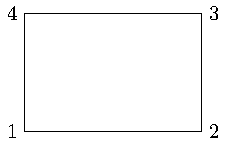
\includegraphics[width=0.25\textwidth]{papers/print/pic/pic_1.pdf}
		\hspace{10mm}
		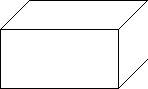
\includegraphics[width=0.25\textwidth]{papers/print/pic/pic_2.pdf}
	\end{minipage}
	\end{center} 

	\begin{center}
	\subsection*{Серия 2. Нормальное завтра. }
	\addcontentsline{toc}{subsection}{\protect\numberline{}Серия 2. Нормальное завтра.}%
	\end{center}

	\epigraph{Whenever groups disclose themselves, or could be introduced, simplicity crystallized out of comparative chaos.}{E. T. Bell}

	%\bf{0.} Пусть $\varphi \colon G \to H$~--- гомоморфизм групп. а) Докажите, что $\Ker{\varphi}$~--- подгруппа в $G$. б) Докажите, что $\Im{\varphi}$~--- подгруппа в $H$. в) Докажите, что $\varphi$ инъективен тогда и только тогда, когда $\Ker{\varphi} = \{ e_{G} \}$. 

	\bf{0.} а) Верно ли, что $C_{2} \times C_{4} \cong C_{8}$? б) Опишите условия, при которых  $\Z/m \times \Z/n \cong \Z/nm$ (и докажите изоморфность в этом случае). 


	\bf{1.} Пусть $G$~--- конечная группа, в которой в точности один элемент $f$ порядка 2. Докажите, что 
	\[
		\prod_{g \in G} g = f.
	\]

	\bf{2.} Пусть $G$~--- группа чётного порядка. Докажите, что в ней есть элемент порядка $2$. 

	\bf{3.} Пусть $g \in G$~--- элемент нечётного порядка. Что можно сказать о порядке $g^2$?

	 \bf{4.}  Пусть $N$~--- подгруппа группы $G$, будем говорить, что она \emph{удовлетворяет свойству $(\cH)$}, если $\forall g \in G \ \forall n \in N$ существует такой $n' \in N$, что $gn = n'g$.

	Для подгруппы $H$ и элемента $g$ будем обозначать $g H = \{ gh \ \vert \ h \in H \}$, а для $R \subset G$ будем обозначать $RH = \{ r h \vert \ r \in R, h \in H \}$.

	а) Докажите, что если $N$ это подгруппа, то
	\vspace{-2mm}
	\begin{enumerate}
		\item $NN = N$. 
		\item $N^{-1} = N$. 
		\item Если $\forall g\in G\  \forall n \in N\colon g n g^{-1} \in N$, то $N$ удовлетворяет свойству $(\cH)$.
	\end{enumerate}

	б) Докажите, что если $N$ удовлетворяет свойству $(\cH)$, то
	\vspace{-2mm}
	\begin{enumerate}
		\item $\forall g \ gN = Ng$.
		\item $(gN)(hN) = (gh)N$ и приведите пример, когда это не так если $N$ не удовлетворяет условию $(\cH)$.
	\end{enumerate}

	в) Пусть $\varphi \colon G \to H$~--- гомоморфизм групп, $N = \Ker{\varphi}$. Докажите, что $N$ удовлетворяет свойству $(\cH)$.

	\bf{5.} Неряшливый преподаватель выписал на доску список из девяти целых чисел, образующих группу по умножению по модулю $91$. К сожалению, он забыл выписать одно из чисел и на доске были выписаны лишь числа $1, 9, 16, 22, 53, 74, 79, 81$. Какое число он забыл написать? 

	\begin{definition} 
		\emph{Моноидом} называется множество $M$ с ассоциативной бинарной операцией и нейтральным элементом.   
	\end{definition}

	\bf{6.} Пусть $M_1, M_2$~--- моноиды. Отображение $\varphi \colon M_1 \to M_2$ назовём \emph{хорошим}, если $\forall a, b \in M_1 \ \varphi(ab) = \varphi(a) \varphi(b)$
	  Верно ли, что если $\varphi$~--- хорошее отображение, то $\varphi(e_{M_1}) = e_{M_2}$?

	 \bf{7.}  Пусть $G, H$~--- группы,  $G \cong H \times G$. Можно ли из этого заключиь, что $H$~--- тривиальная группа. (\emph{Подсказска.} Нет! Попробуйте построить контрпример.)

	 \bf{8.} Докажите, что $(\Q, +)$ не может быть представлена в виде произведения двух нетривиальных групп.

	 \begin{center}
	 	\subsection*{Серия 3. Действию время, а потехе час. }
	 	\addcontentsline{toc}{subsection}{\protect\numberline{}Действию время, а потехе час. }%
	 \end{center}

	\epigraph{Двадцать две основные буквы: Бог их нарисовал, высек в камне, соединил, взвесил, \emph{переставил} и создал из них все, что есть,~--- и все, что будет.}{Сефер Йецира}

	\bf{0.} Докажите, что $G \times H \cong H \times G$.

	\bf{1.} Пусть $A, B$~--- абелевы группы. Обозначим за $\mathrm{Hom}(A, B)$ множество гомоморфизмов из $A$ в $B$. Задайте на $\mathrm{Hom}(A, B)$ структуру абелевой группы. 

	\bf{2.} Докажите формулу для числа сочетаний $\binom{n}{k}$ при помощи действия группы на множестве. 

	\bf{3.} а) Докажите, что $\sum_{\pi \in S_n} |\mathrm{fix}(\pi)| = n!$. б) Пусть группа $G$ транзитивно действует на множестве $X$. Каково среднее значение числа неподвижных точек элементов по всей $G$, то есть 
	\[
		\frac{1}{|G|}\sum_{g \in G} |\mathrm{fix}(g)|. 
	\]


	\bf{4.} а) Мальчик Вася нарисовал на бесконечном листе бумаги такой концептуальный рисунок: 
	\[
		\ldots \ \Gamma \ \Gamma \ \Gamma \ \Gamma \ \Gamma \ \Gamma \ \Gamma \ \Gamma \ \Gamma \ \Gamma \ldots
	\]
	Найдите группу симметрий этого рисунка. 

	б) то же самое, но для рисунка 

	\[
		\ldots \ \mathrm{D} \ \mathrm{D} \ \mathrm{D} \ \mathrm{D} \ \mathrm{D}\ \mathrm{D} \ \mathrm{D} \ \mathrm{D} \ \mathrm{D} \ \mathrm{D}\ldots
	\]

	\noindent\bf{Комментарий.} в данной задаче мы ищем \emph{только те симметрии, которые переводят соседние буквые в соседние}. И, отметим, что буквы стоят на \emph{одинаковом} расстоянии. 

	\begin{definition} 
		Симметрической группой $S_{X}$ на множестве $X$ называется группа биекций $X \to X$.
	\end{definition}

	\bf{5.} Докажите, что любая группа $G$ реализуется, как подгруппа в некоторой симметрической группе (т.е. симметрической группе какого-то множество). \emph{Подсказка.} Если у нас есть инъективный гомоморфизм $\varphi\colon G \to H$ по очевидным причинам $\mathrm{Im}{\varphi} \cong G$ и мы можем отождествить образ с самой группой $G$. 

	\begin{definition} 
		\emph{Дробно-линейным} преобразованием называется функция $f\colon \HH^2 \to \HH^2$ вида 
		\[
			f(z) = \frac{az + b}{cz + d}, \quad a, b, c, d \in \R,\  ad - bc = 1.
		\]
		Здесь $\HH^2 = \{ z \in \C \ \vert \ \Im{z} > 0 \}$. 
	\end{definition}


	\bf{6.} Докажите, что дробно-линейные преобразования образуют группу относительно композиции.

	\begin{center}
		\subsection*{Серия 4. С приложениями теории групп.}
		\addcontentsline{toc}{subsection}{\protect\numberline{}Серия 4. С приложениями теории групп.}%
	\end{center}

	\epigraph{Я не имею права задерживать нормального человека в лечебнице. Тем более что у меня и мест не хватает. И я вас сию же секунду выпущу, если только вы мне скажете, что вы нормальны. Не докажете, поймите, а только скажете. Итак, вы — нормальны?}{Михаил Булгаков, ‘Великий Канцлер’}

	\bf{0.} Докажите, что действие группы на себя левыми трансляциями свободно.  

	\bf{1.} Докажите, что подгруппа индекса 2 нормальна. 

	\bf{2.} Пусть $G$~--- группа поворотных гомотетий плоскости с центром в точке $O$, а $H$~--- подгруппа поворотов плоскости с центром в точке $O$. а) Докажите, что $H$~--- нормальная подгруппа. б) Вычислите $G/H$.

	\begin{definition} 
		Пусть $G$~--- группа. \emph{Группой автоморфизмов $G$} называется группа изоморфизмов из $G$ в себя. 
	\end{definition}

	\bf{3.} а) Вычислите группу автоморфизмов $\mathrm{\Aut}(\Z)$. б) Вычислите группу автоморфизмов $\mathrm{\Aut}(C_{p})$. 

	\bf{4.} Докажите, что матрицы  $\begin{pmatrix} a & b \\ c & d \end{pmatrix}$ где $a, b, c, d \in \R, \ ad - bc = 1$ образуют группу по умножению. 

	\bf{5.} Пусть $n \in \N$~--- натуральное число. Постройте группу, в которой есть такие элементы $a$ и $b$, что 
	\[
		\ord{a} = \ord{b} =  2, \quad \ord{ab} = n.
	\]
	
	\bf{6.} Для любого $n \ge 3$ постройте граф, группа симетрий которого изоморфна $\Z/n$.

	\bf{7.} Определите группу симметрии внешней оболочки поперечного среза вируса иммунодефицита человека, показанного ниже.

	\begin{center}
		
\includegraphics[scale = 0.3]{papers/print/pic/pic_3.png}
	\end{center}

	\bf{8.} Вася нарисовал на  плоскости  клетчатый прямоугольник $n \times m$. Сколькими  с точностью то отражения относительно горизонтальной и вертикальной осей способами он может раскрасить его в $k$ цветов?

	\begin{center}
		\subsection*{Серия 5. А теперь к делу. }
		\addcontentsline{toc}{subsection}{\protect\numberline{}Серия 5. А теперь к делу. }%
	\end{center}

	\epigraph{Однажды, сидя под деревом бодхи, Сиддхартха достиг просветления. Ему открылась истина о природе страдания и пути к освобождению от него. Он понял, что основной источник страданий~--- это желание и привязанность к материальным вещам. Из этого понимания родилось учение о восьми благородных истин и пути к просветлению~--- Изначальному Учению.}{Об автоморфизмах деревьев.}

	\bf{0.}  Вычислите фаткторгруппу группы симметрий пятиугольника по подгруппе поворотов. 

	\begin{definition} 
		Пусть $G$~--- группа. \emph{Коммутатором} элементов $g$ и $h$ называется $[g, h] = g h g^{-1} h^{-1}$.
	\end{definition}

	\bf{1.} Для группы $G$ обозначим через $[G, G]$ подгруппу $\langle [g, h] \ \vert \ g, h \in G \rangle$. а) Докажите, что $[G, G] \trianglelefteq G$, б) Докажите, что $G/[G, G]$~--- абелева группа. 

	\bf{2.} Пусть $G$~--- группа, $H, K$~--- её подмножества. а) Докажите, что $K \le H, \ H \le G \implies K \le G$. б) Пусть $K \trianglelefteq  H, \ H \trianglelefteq  G$. Верно ли, что $K \trianglelefteq  G$?

	\bf{3.} Пусть $H$ и $K$~--- подгруппы в $G$. Докажите, что 
	\[
		|HK| = \frac{|H|\cdot|K|}{|H \cap K|}	
	\]
	\begin{definition} 
		Обозначим группу матриц $\begin{pmatrix} a & b \\ c & d \end{pmatrix}$, где $a, b, c, d \in \R$ и $ad - bc = 1$ за $\mathrm{SL}_{2}(\R)$.
	\end{definition}

	\bf{4.} Проверьте, что $\mathrm{SL}_{2}(\R)$ это действительно группа и постройте изоморфизм в группу дробно-линейных преобразований $\HH^2$. 

	Во всех задачах ниже $G$~--- транзитивная на уровнях подгруппа $\mathrm{Aut}(X^*)$.

	\bf{5.}  Докажите, что для любой вершины $v \in X^n$ её стабилизатор  $\Stab(v)$~--- это подгруппа индекса $|X|^n$ в группе $G$. 

 	\bf{6.} Докажите, что для любой вершины $v \in X^*$ и любого $g \in G$ жесткий стабилизатор $G[v]$ обладает следующим свойством: 
 	\[
 		G[g(v)] = g G[v] g^{-1}.
 	\]

 	\bf{7.} Докажите, что если слово $v$ является началом слова $u \in X^*$, то $\Stab(u) \le \Stab(v)$ и $G[u] \le G[v]$.

 	\bf{8.} Докажите, что а) уровневые стабилизаторы $\Stab(n)$ являются нормальными подгруппами конечного индекса в $G$. б) Докажите, что  
 	\[
 		\bigcap_{n \ge 1} \Stab(n) = \{ e \}.
 	\]

 	\begin{center}
 		\subsection*{Серия 6. Разгрузочное. }
 		\addcontentsline{toc}{subsection}{\protect\numberline{}Серия 6. Разгрузочное. }%
 	\end{center}

	%\epigraph{Свободная группа с двумя образующими~--- это не группа, это просто набор слов.}{Анатолий Моисеевич Вершик}

	\epigraph{Все мы по-разному смотрим на понятие группы. Физики смотрят на группы, как на группы Ли, как на непрерывные группы. Я беседовал с одним очень продвинутым физиком, пытался ему объяснить, что такое свободная группа на двух образующих, очень трудно было!}{Роман Валерьевич Михайлов}

	Напомним, что $\mathrm{Aut}{X^*}$~--- группа автоморфизмов корневого дерева $X^*$, а $S_{X}$~---  симметрическая группа на множестве $X$.

	Пусть $g\colon X^* \to X^*$~--- \bf{эндоморфизм} корневого дерева $X^*$. Рассмотрим поддеревья $v X^*$ и $g(v) X^*$. Тогда $g$ индуцирует морфизм корневых деревьев $g\colon v X^* \to g(v) X^*$ (\bf{нарисуйте картинку!}). 

	Заметим, что корневое поддерево $v X^*$ естественно изоморфно \bf{всему} дереву $X^*$ (вспомните, что изоморфизм задаётся отображением $vw \mapsto w$). Тот же факт $g(v)X^*$. Отождествляя оба поддерева $v X^*$ и $g(v) X^*$ с $X^*$ мы получаем отображение $g\vert_{v} \colon X^* \to X^*$, однозначно определённое формулой 
	\[
		g(vw) = g(v) g\vert_{v}(w).
	\]

	Мы будем называть эндоморфизм $g\vert_{v}$ \emph{сужением} $g$ на вершину $v$.

	\bf{0.} Докажите, что выполняются следующие свойства сужения: а) $g\vert_{v_1 v_2} = g\vert_{v_1}\vert_{v_2}$, б) $(g_1 \cdot g_2)\vert_{v} = g_1\vert_{g_2(v)} \cdot g_2\vert_{v}$. 

	\bf{1.} Постройте изоморфизм 
	\[
		\mathrm{Aut}{X^*} \to S_{X} \wr \mathrm{Aut}{X^*}. 
	\]

	\bf{2.} Пусть $H$~--- группа, действующая на конечном множестве $X$, а $G$~--- произвольная группа. Представьте $H \wr G$ в виде (нетривиального) полупрямого произведения групп. 

	 Хоть эта задача и не сложная, в ней оцениваются любые продвижения! 

	 \bf{3.} Опишите группу аффинных преобразований прямой $\R$ (т.е. функция вида $ax + b, \ a, b \in \R$, как полупрямое произведение двух групп. 

	 \begin{center}
	 \subsection*{Серия 7. Папа Карло тоже действовал на дереве\ldots }
	 \addcontentsline{toc}{subsection}{\protect\numberline{}Серия 7. Папа Карло тоже действовал на дереве\ldots }%
	 \end{center}

	\epigraph{Целый новый ряд мыслей безнадежных, но грустно-приятных в связи с этим дубом возник в душе князя Андрея. Во время этого путешествия он как будто вновь обдумал всю свою жизнь и пришел к тому же прежнему, успокоительному и безнадежному, заключению, что ему начинать ничего было не надо, что он должен доживать свою жизнь, не делая зла, не тревожась и ничего не желая.}{Л.Н. Толстой, <<Война и мир>>}

	В этой сери задач $\mathbf{G}$~--- группа Григорчука, а $a, b, c, d$~--- как в лекции. 

	\bf{1.} а) Проверьте, что $b, c, d$ имеют порядок 2, коммутируют друг с другом и удовлетворяют групповому тождеству  $b \cdot c \cdot d = 1$. б) Выведите отсюда, что $\langle b, c, d \rangle \cong \Z_{2}^2$. в) Докажите, что $\mathbf{G} = \langle a, b, c, d \rangle$ 3-порожденная. 
	
	\bf{2.} а) Проверьте, что в группе $\mathbf{G}$ выполняются соотношения 
	\[
		(ad)^4 = (ac)^8 = (ab)^{16} = 1.
	\]
	б) Выведите отсюда, что подгруппы $\langle a, b \rangle$, $\langle a, c \rangle$, $\langle a, d \rangle$ группы $\mathbf{G}$ конечны. 

	\bf{3.} Вася переписывает элементы группы $\mathbf{G}$ по следующимс правилам
	\[
		\xi\colon a \mapsto aba, \ b \mapsto d, \ c \mapsto b, \ d \mapsto c.
	\]
	а) Помогите Васе построить последовательность элементов $\mathbf{G}$ такую, что $x_1 = a$ и $\forall i \ge 1 \ x_{i + 1} = \xi(x_{i})$. б) Докажите, что все элементы $x_i$ различны. в) Выведите из этого, что  $\mathbf{G}$ бесконечна.


	\begin{center}
	\centerline{\bf{Серия 8.  Растём над собой\ldots }}
	\addcontentsline{toc}{subsection}{\protect\numberline{}Серия 8.  Растём над собой\ldots }%
	\end{center}

	\epigraph{Свободная группа с двумя образующими~--- это не группа, это просто набор слов.}{Анатолий Моисеевич Вершик}

	\bf{0.} Чему изоморфна группа $\langle a, b, c \ \vert \ a^{5} = 1, \ b^{17} = 1, \ c^{239} = 1, \ [a, b] = 1, \ [a, c] = 1 , \ [b, c] = 1 \rangle$.

	\bf{1.} В группе $G$ выполнены соотношения $a^2 = b^5 = (ab)^4$ и $(a b^{-2} a b^2)^2 = a^2$. Докажите, что $(ba)^4 = 1$. 

	\bf{2.}  Мама отправила Васю в магазин <<Мир теории групп>>, чтоб он принёс полезную в быту группу, но написала в списке не её название, а задание образующими и соотношениями:
	\[
		G = \langle \eta_1, \ldots, \eta_{n - 1} \ \vert \ \eta_j^2 = 1, \ (\eta_j \eta_{j + 1})^3, \ \eta_j \eta_{\ell} = \eta_{\ell} \eta_{j} \ \forall \ j, \ell \colon |j - \ell| > 1 \rangle. 
	\]

	Помогите Васе понять, какую группу ему надо купить в магазине. 

	\bf{3.} Пусть $G$~--- транзитивная на уровнях подгруппа в группе автоморфизмов $\mathrm{Aut}(X^*)$, а $w \in X^*$. Докажите, что если $h \in G[w]$ и $g(w) \neq w$, то $[h, g] \neq 1$. 

	\bf{4.} Рассмотрим в группе Григорчука $\mathbf{G}$ следующее правивло переписывания 
	\[
		\tau\colon a \mapsto a c a, \ c \mapsto c d, \ d \mapsto c.
	\]
	Докажите, что $\tau^i(ad)^4 = 1$
	
	 	
	\bf{5.} Рассмотрим группу $\Z = \langle r, s \rangle$, где $0 < r < s$. Докажите, что для достаточно больших $n$ сферическая функция роста будет иметь вид  $s_{\Z}(n) = 2s$.  

	\bf{6.} Пусть $G$~--- произвольная конечнопорожденная группа. Докажите, что для её шаровой функции роста выполнено неравенство
	\[
	 	b(n + m) \le b(n)b(m).
	 \] 
	 б) выведите из этого, что $\lim\limits_{n \to \infty} (b(n))^{1/n}$ существует и конечен.

	  \bf{7.} Заведём на множестве функций $f\colon \N \to \R_{+}$ такое отношение эквивалентности 
	 \[
	 	f \approx g \Leftrightarrow  f \preceq g \text{ и } g \preceq f,
	 \]
	 где $f \leqslant g$, если $\exists A \ge 1\colon f(n) \le A \cdot g(An)$ для достаточно больших $n$. Убедитесь, что это в самом деле отношение эквивалетности. 
	

	


\end{document}